\section{A \Cyclus Model of Nuclear Weapon Pursuit}
\label{s_methods}

We have applied the factors correlated to pursuit of nuclear weapons in a regional model of state interactions using \Cyclus\cite{huff_open_2011,huff_fundamental_2016,gidden_agent-based_2013}.  The \gls{CNERG}\footnote{http://cnerg.github.io/} group at the University of Wisconsin has developed the \Cyclus\footnote{http://fuelcycle.org/} nuclear fuel cycle simulator to model all aspects of the nuclear fuel cycle in a flexible way \cite{cyclus_v1_3}.  \Cyclus has three key features: it is \textit{agent-based}, it tracks \textit{discrete materials}, and it incorporates \textit{social and behavioral interaction models}\cite{jennings_agent-based_2000, taylor2014agent}. This design allows customized facilities and institutions to engage in dynamic decision-making based on their preferences, needs, or political constraints across a wide range of scenarios.  A specific agent might have preferences based on material composition, physical proximity between facilities, or preferred trading partners, which are implemented in a region-institution-facility hierarchy that enables economic modeling \cite{oliver_geniusv2:_2009}.

\subsection{The Forward Model}

The region-institution-facility design has been used to develop the \gls{NWPM}. This forward model features two custom archetypes, an interaction region (InteractRegion) and a state institution (StateInst) \TODO{CITE mbmore}.  The state institution represents the a nation-state.  It includes time-dynamic information about each of the pursuit factors. The interaction region is an omniscient presence in the simulation that tracks weapon status as well as interactive pursuit factors such as conflict(as described in section \ref{section:s_pe}), and communicates that factor to each individual state. 

Each of the motivating factors is defined for every state in a time dynamic way. Individual factors must have values between 0-10. There are several tim dynamics currently available in the model: constant, linear growth or decline, step-function (at either a specified or a randomly chosen time), or power-law.  These functions enable modeling of characteristics such as growth in military spending, development of new technologies such as enrichment, and sudden changes such as to governing structure or inter-state conflict.  At each timestep, the state combines all of these factor values into a pursuit score using the weighted linear equation defined in section \ref{section:s_factors}.

 \subsection{Likelihood}

\begin{figure}%[htbp!]
\begin{center}
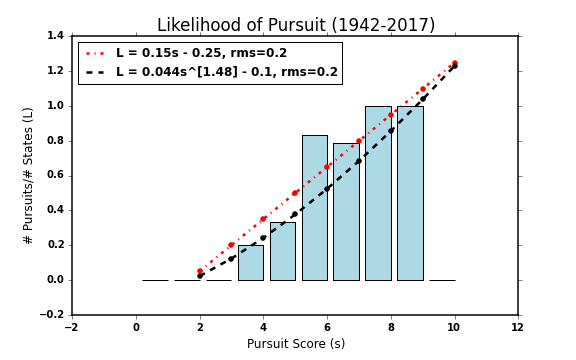
\includegraphics[scale=0.8]{./figs/pe_likely.png}
\end{center}
\caption{Fraction of states with any nuclear technology (dataset from \ref{s_factors}) that pursued weapons at some point in the last 75 years, given their pursuit scores. The black power-law curve is a better fit to the data compared with the red weighted linear fit.}
\label{fig:likely}
\end{figure}
 
The score is then converted into a likelihood that the state will pursue a weapon. The relationship between pursuit score and likelihood of pursuing a weapon has been characterized using historical data of the 42 states that have developed nuclear technology since 1942.  \ref{fig:likely} shows the fraction of states with a given pursuit score that pursued a weapon during that time. A power-law (red) provides a better fit to the data compared with a weighted linear fit (black).  This data represents the total likelihood integrated over the course of 75 years ($T$). \ref{eqn:likely_eqn} is used to convert to the likelihood of pursuit $L$ in any given year, given a pursuit score $s$.

\begin{equation}
L = 1 - (1 - s)^{1.0/T}
\label{eqn:likely_eqn}
\end{equation}

In the \gls{NWPM} forward model, each state's score is converted to a likelihood of pursuit at that timestep using \ref{eqn:likely}. The actual conversion is bounded using two heavy-side functions such that scores below a lower threshold (e.g. 4) are forced to a likelihood of zero, while scores above an upper threshold (e.g. 9) are forced to the value of the score at the threshold.   A random number generator is used given the likelihood to determine whether or not the pursuit event occurs. If the determination is for pursuit to occur, the state deploys a secret enrichment facility. If a state is already pursuing a weapon, then the model determines whether it succeeds in acquiring a weapon at that timestep using a median time to acquire of 20 years, based on historical data for states that have acquired weapons\TODO{WHAT IS EXACT MEDIAN FOR STATES THAT HAVE SUCCEEDED?}. On the timesteip in which a state succeeds in acquiring a weapon, highly enriched uranium is shipped out of the secret enrichment facility.

\subsection{Limitations of the Historical Data}
The use of historical data to develop a forward model has several limitations. One set of limitations could be improved with a larger historical dataset.  Historical scores for non-nuclear states have not been calculated. Due to the influence of nuclear technology, a non-nuclear state could theoretically have a maximum pursuit score of 7. Considering that the majority of states that have high potential military spending and major historical conflicts have already been incorporated, this further reduces the potential maximum score to below 5, even if all other factors were maximized.  A large fraction of states in the world are have scores on the order of 1-3.  This large set of missing historical data, heavily weighted to the low score side, would reduce the likelihood of higher-score states from pursuing.  The database could also be improved by collecting historical data for many years around dates of pursuit and acquisition rather than just for a single year. This analysis has identified factors that are correlated to weapons programs but there is insufficient data to confirm causal relationships.   

This model is intrisnically limited by the small sample size and the degree to which the global landscape changes over time. With only 10 states that have acquired nuclear weapons throughout history, there is large uncertainty in any quantatitative analysis. Additionally, while conflict has been captured in a crude way, it is difficult to develop a parameterization with enough nuance to capture the varying impact of conflict under paradigms such as World War II, the Cold War, or post-9/11.

